%!TEX root = cscw2019-comic.tex
\section{Discussion}
\label{sec:Discussion}
We will first summarize our findings and discuss experimental variations. Then, we will propose a framework for algorithmically synthesizing persuasive messages into the abstract comic form, discuss design implications, and identify limitations.

\subsection{Experiments: Findings and Alternative Contexts}
\label{sub:Experiments: Findings and Alternate Contexts}

From asking individuals to act to appealing for charitable donations, text messages have been widely used in simulating behaviors. Scholars from psychology have shown how variations in the construction of text messages alter decisions. We explored and examined the role of the abstract comic form, a highly expressive, affective medium in communicating persuasive messages. To test the effectiveness of abstract comic persuasive messages, we persuaded individuals to make online charitable donations, a common public good dilemma. In the dilemma, due to the non-exclusive and non-rivalrous nature of public goods, persuading individuals to contribute is hard and crucial. Also, online charitable donation task not only avoids confounding factors such as habit formation which exists in other persuasion tasks such as exercise and healthy diet but also assures the ecological validity of our study as charity and organizations often solicit donations online. In our study, we compared the persuasive power of text messages, comic messages, and comic messages with social proof in asking charitable donations to public health research (e.g., the Organization for Autism Research).

\begin{description} [leftmargin=\parindent,topsep=0pt,partopsep=3pt,parsep=0pt,itemsep=3pt, listparindent=\parindent]
    \item[Comic vs. Plain Text:] Our results show that study participants prefer persuasive messages in abstract comic form over plain text. When making the charitable donation between $\$0$ to $\$5$, study participants donated $\$ 0.86$ more if they read the persuasive message in an abstract comic form (see~\Cref{fig:robustcontrasts}, fourth column). The results demonstrate the persuasive power of abstract comic in stimulating behaviors in pro-social decisions. Our findings are consistent with prior research on visual stimuli in persuasion and the benefits of comics in communication. One potential explanation is that study participants were more attracted by the comic strip and projected themselves onto the character. When the projection happens, the persuadee may be able to digest the information better which stimulated them to donate more to the Organization for Autism Research. 
    
    \item[Social Proof Condition:] When comparing between the comic condition and comic with the social proof condition, although study participants who read the comic with social proof donated more on average (\$0.19 more) that the comic only condition, our analysis results do not indicate a significant difference between the two conditions (see~\Cref{fig:robustcontrasts}, third column). 
    % Although the use of social proof showed a significant impact on other forms of persuasive messages (e.g., plain text), in the abstract comic messages, the effect is not substantial. 
    We can identify two explanations. First, it is possible that the design of our comic strip did not signify the idea of social proof strongly---we simply introduced the pilot study statistic in the text bubble. Other comic designs, e.g., adding other donators as comic characters, may make the social proof more salient. Another potential explanation is that the influence from other study participants is not strong enough. As \textcite{goldstein2008room} discovered hotel towel re-use study, stronger the relationship between the subject and the reference group of individuals from whom the experimenters compute the statistic for the social norm, the message is more persuasive. It is possible that the relationship between the AMT subjects may be weaker than the study in \textcite{goldstein2008room}'s towel re-use study.

    We conjecture that using a person's social network as part of the social proof (after seeking consent, for example, to use the person's Facebook profile information) may increase the contribution, but needs further research. We know from Cialdini's seminal work on persuasion that knowledge of friends performing similar behavior is persuasive. We know from \textcite{small2007sympathy}'s work on charitable donation that named entities are more powerful in persuasion than abstract statistics (e.g. ``Jane Doe is a hurricane survivor; please help'' vs. ``3000 people homeless due to the hurricane; please help''). If the person has given consent, a charity could find out in real time, the Facebook friends of the person who has loaded the web-page, and compute the fraction who have donated and use that number in the social proof. Or to use tie-strength \cite{Gilbert}, if available and name the closest friend who has donated to the charity, in the social proof message. However, we know from recent work \cite{eslami2018communicating} that when advertisers display information that subjects find ``creepy'' (as demonstration of knowledge by the charity of the subject's closest friend, of even statistics of the person's Facebook friends circle contributions), the subjects may find the charity less trustworthy and may donate less.
    
    % discovered that the closer the relationship is, the stronger the social proof will be, comparing to the neighbors or people stayed at the same room in \textcite{Cialdini2004} and \textcite{goldstein2008room}'s work, the relationship among participants in our study may be much weaker. So, we did not observe a strong influence from abstract comics with social proof.
    \item[Donation Amount:] Another natural question to ask is whether the maximum donation amount of  \$5  in our study has any influence on our findings (e.g., will people make the same donation decision if they can donate more?).  Prior studies in behavioral economics suggested that small-stake experiment in developed countries can be replicated in developing countries where the stake becomes a significant portion of participants' weekly income \cite{binswanger1980attitudes,binswanger1981attitudes,kachelmeier1992examining}. Additionally, \textcite{post2008deal} showed that the results from small-stake experiments would hold with higher stakes in developed countries as well. Those results seem to suggest that our findings will hold with higher donation amount. However, the best way to confirm is through actual experiments. 
    \item[Other Media Forms:] While a direct comparison between the comic form and images and videos is beyond the scope of the paper, we discuss two advantages of using the abstract comic to persuade.There are two points to consider: the ease of making a connection with a viewer (the abstract comic form vs. images or video); infrastructure to create tailored messages. First, as \textcite{mccloud2011making} points out, when using the abstract comic form, the reader projects themselves onto the character. A concrete and detailed representation of the person in the comic causes the reader develops a sense of the ``other'' - that is, they are viewing someone else enacting a scene. Using images and videos with actual human models, will create a sense of the ``other'' for the viewer, and then the images/video need to connect with the viewer through demographic, cultural and local cues. For example, in advertising, to allow for recipients of ads to identify with the message context, advertisers try to ensure that the models who appear in images match the target demographic. In contrast, when viewing an abstract comic, the reader fills in the gaps with their own characteristics, and they see themselves as the protagonist. Second, our infrastructure (discussed next in~\Cref{sub:framework}) makes it straightforward for a charity to compose a multi-panel abstract comic. The infrastructure to create tailored imagery and videos may be expensive for the charity. Today, advertisers tailor the imagery (usually the individual in the image) in online banner ads (embedded on a web page) to the demographics of the person viewing the ad. Matching the demographics requires that advertisers access the information stored in a browser cookie against third-party information about the person in real-time. This real-time switching of imagery is expensive: it requires a manually curated image collection corresponding to individuals matching to different demographic segments of interest. And, to personalize the message (e.g. with the social norm), they would need to have the infrastructure to compose the message on the fly. Furthermore, algorithmic synthesis of persuasive, personalized videos is more challenging. One possibility that we do consider as part of future work: animations that involve the abstract comic form.
    %\textcolor{red}{When considering persuasive messages in non-textual forms, besides abstract comics, graphical representation and video messages are often discussed. Although the scope our study is not to compare the persuasive power between comics and other non-textual forms, the abstract nature of the comics allows low-cost synthesizing comparing to other non-textual forms, especially when the original message is personalized, which makes the abstract comic persuasive message worth to consider.}
    \item[General Experimental Flow:] Consider three online charitable donation scenarios related to how the charitable organization knows the person asked to make a donation. In each case, consistent with prior work ~\cite{pessemier1977willingness}, the charity needs to establish context. There are three ways to consider.
    
    First, the person may be familiar with the charity through their lived experience. For example, in the case of Wikipedia, the person may be someone who uses the site frequently. A person who regularly uses the Wikipedia site is unlikely to need a video describing Wikipedia benefits. In such cases, we envision using the three-panel comic instead of the desktop banner ad that Wikipedia uses at the moment.
    
    Second, the person may be a member of the charity or non-profit (e.g. museums).For 501(c) non-profit organizations with memberships, that recognize that a member has logged onto the organization website, again detailed context may be less necessary and they could use the three-panel comic along with their regular ask page, along with social proof describing the fractions of other members who have contributed.
    
    Third, the person may not know the charity. For charities who need to ask for donations without the benefit of either lived experience or of memberships, need to establish context from scratch. They may establish context through videos, a page with text and images or even a physical mailer. After watching the videos or reading the page, they may show the person visiting the page the comic. For the physical mailer, the charity would include its usual textual description and imagery followed by the abstract three-panel comic. After the comic panel, they may direct the person opening the mailer to a web-page to make a contribution.
    
    For the first two scenarios, a charitable organization (e.g. Wikipedia) can determine regular use of its website or determine if the person visiting the web-page is an organization member through the use of advertising cookies.

    
    %\hs{How might a charity use our findings? In general, consistent with prior work on donations~\cite{pessemier1977willingness} that indicates that an individual's prior knowledge of the purpose may influence their donation behavior, the charity first needs to establish common grounding with a potential donor and then make the request. In the present study, the video plays helps the experimental subjects familiarize themselves with the charity. The role of the video is to provide context, grounding the subject with the purpose of the charity. } 
    
    %\hs{In general, a person may establish grounding with the charity in other ways beyond an introductory video or a web-page with descriptions, including through their lived experience and through membership. Consider two examples. First, a person who regularly uses the Wikipedia site is unlikely to need a video describing Wikipedia benefits.  In such cases, one may envision using a multi-panel comic instead of the desktop banner ad that Wikipedia uses at the moment.  Second, for 501(c) non-profit organizations with memberships (e.g. museums), that recognize that a member has logged onto the web-site, again detailed context may be less necessary and they could use the three panel comic along with the regular ask page, along with social proof describing the fractions of other members who have contributed.  A charitable organization (e.g. Wikipedia) can determine regular use of its website or determine if the person visiting the web-page is a organization member through the use of advertising cookies.} 
    
    %\hs{For charities who need to ask for donations of an individual without either experience with the charity or is not a member, the charity needs to establish context. They may establish context through videos, a page with text and images or even a physical mailer. After watching the videos or reading the page, they may then show the person visiting the page the comic. For the case of physical mailer, the charity would include its usual textual description and imagery followed by the abstract multi-panel comic. After the comic panel, they may direct the person opening the mailer to a web-page to make a contribution.}
\end{description}




% \textcolor{red}{We conjecture that using a person's social network as part of the social proof may increase contribution, but needs further research. We know from Cialdini's seminal work on persuasion that knowledge of friends performing similar behavior is persuasive. We know from \textcite{small2007sympathy}'s work on charitable donation that named entities are more powerful in persuasion than abstract statistics (e.g. "Jane Doe is a hurricane survivor; please help" vs. "3000 people homeless due to hurricane; please help").It ought to be straightforward for a charity to find out in real time, the Facebook friends of the person who has loaded the web-page, and compute the fraction who have donated and use that number in the social proof. Or to use tie-strength \cite{Gilbert}, if available and name the closest friend who has donated to the charity, in the social proof message. However, we know from recent work \cite{eslami2018communicating} that when advertisers display information that subjects find "creepy" (as demonstration of knowledge by the charity of the subject's closest friend, of even statistics of the person's Facebook friends circle contributions), the subjects may find the charity less trustworthy and may donate less.}

% Another natural question to ask is whether the maximum donation amount of  \$5  in our study has any influence on our findings (e.g., will people make the same donation decision if they can donate more?).  Prior studies in behavioral economics suggested that small-stake experiment in developed countries can be replicated in developing countries where the stake becomes a significant portion of participants' weekly income \cite{binswanger1980attitudes,binswanger1981attitudes,kachelmeier1992examining}. Additionally, \textcite{post2008deal} showed that the results from small-stake experiments would hold with higher stakes in developed countries as well. Those results seem to suggest that our findings will hold with higher donation amount. However, the best way to confirm is through actual experiments. 

% \textcolor{red}{While a direct comparison between the comic form and images and videos is beyond the scope of the paper, there are two points to consider, when comparing the comic form, to images and video. First, the abstract comic form used in our experiment allows the reader to project themselves onto the comic character. Our infrastructure (discussed in section x) makes it straightforward for a charity to compose a multi-panel  abstract comic. We plan to make the infrastructure publicly available as open source software after publication,Second, to allow for recipients of ads to identify with the message context, advertisers like to ensure that the models who appear in images match the target demographic. Today, advertisers tailor the imagery (usually the individual in the image) in online banner ads (embedded on a web page) corresponding to the demographic of the person viewing the ad. Matching the demographic requires the advertisers to access the information stored in a browser cookie against third-party information about the person. This real-time switching of imagery is expensive: it requires a manually curated image collection corresponding to individuals matching to different demographic segments of interest. Furthermore, to personalize the message (e.g. with the social norm), they would need to have the infrastructure to compose the message on the fly. Furthermore, algorithmic synthesis of persuasive videos is more challenging.Thus, synthesizing personalized images and videos tailored to the individual may be expensive to generate for a charity. In contrast, they could use our open source software to create an abstract comic for persuasion.}
%\textcolor{red}{When considering persuasive messages in non-textual forms, besides abstract comics, graphical representation and video messages are often discussed. Although the scope our study is not to compare the persuasive power between comics and other non-textual forms, the abstract nature of the comics allows low-cost synthesizing comparing to other non-textual forms, especially when the original message is personalized, which makes the abstract comic persuasive message worth to consider.}

% Although in our study, the persuasive goal is making charitable donation decisions, we believe our findings suggest future research on longitudinal behavior change (e.g., health) via the abstract comic. 

 \subsection{Framework for Algorithmically Synthesized Abstract-Comic Persuasive Messages}
 \label{sub:framework}
 
Our study showed the persuasive power of abstract comics in encouraging people to make pro-social decisions. However, one drawback of using visual stimulus in persuasion is cost during the creation process. Although compared to creating other persuasive visual stimuli such as videos or complex graphical illustration, the simplicity of abstract requires less effort, the creation process is not easy. In this section, we propose a framework that allows full/semi- automatic generation of abstract persuasive messages and identify crucial features that need to be addressed in future work. We believe such a tool will lower the barrier for the persuader to take advantage of the abstract comic (as demonstrated in our study) in encouraging individuals to act in public good dilemmas.

In our study, we created a comic generator with existing packages including ``cmx.io'' \cite{cmx.io} and ``rough.js'' \cite{rough.js} to generate the three-panel abstract comic strip. With several pre-defined character gestures (see~\Cref{figur:figures}), the generator only requests the text input from the persuader to create the comic message.  

We believe the comic generator built in this study can be further developed as a framework for algorithmic synthesis. Now, we identify crucial features that need to be addressed in future research. First, the framework should be able to automatically select the character gesture that best fit the persuasive message's context. For example, when the message receiver was told good news, his/her gesture should reflect that conflict. The appropriate mapping will create a natural and coherent comic message which is the key for an expressive message. We need future research to realize such a method. Second, the framework should be able to use other abstract comic elements, such as inter-character distance and shading, to create persuasive comics. To achieve this feature, we need to understand how different elements affect the persuasiveness of the abstract comic messages. Third, the framework should be able to personalize the persuasive comics by using persuadee's behavioral data to inform comic contents. We could derive the statistics for the social proof from the behaviors of friends and the data from a person's own activity.

\begin{figure}[t]
    \centering
    \begin{tabular}{cc}
        \subfloat[Gestures for positive framed messages]{\label{figur:1a}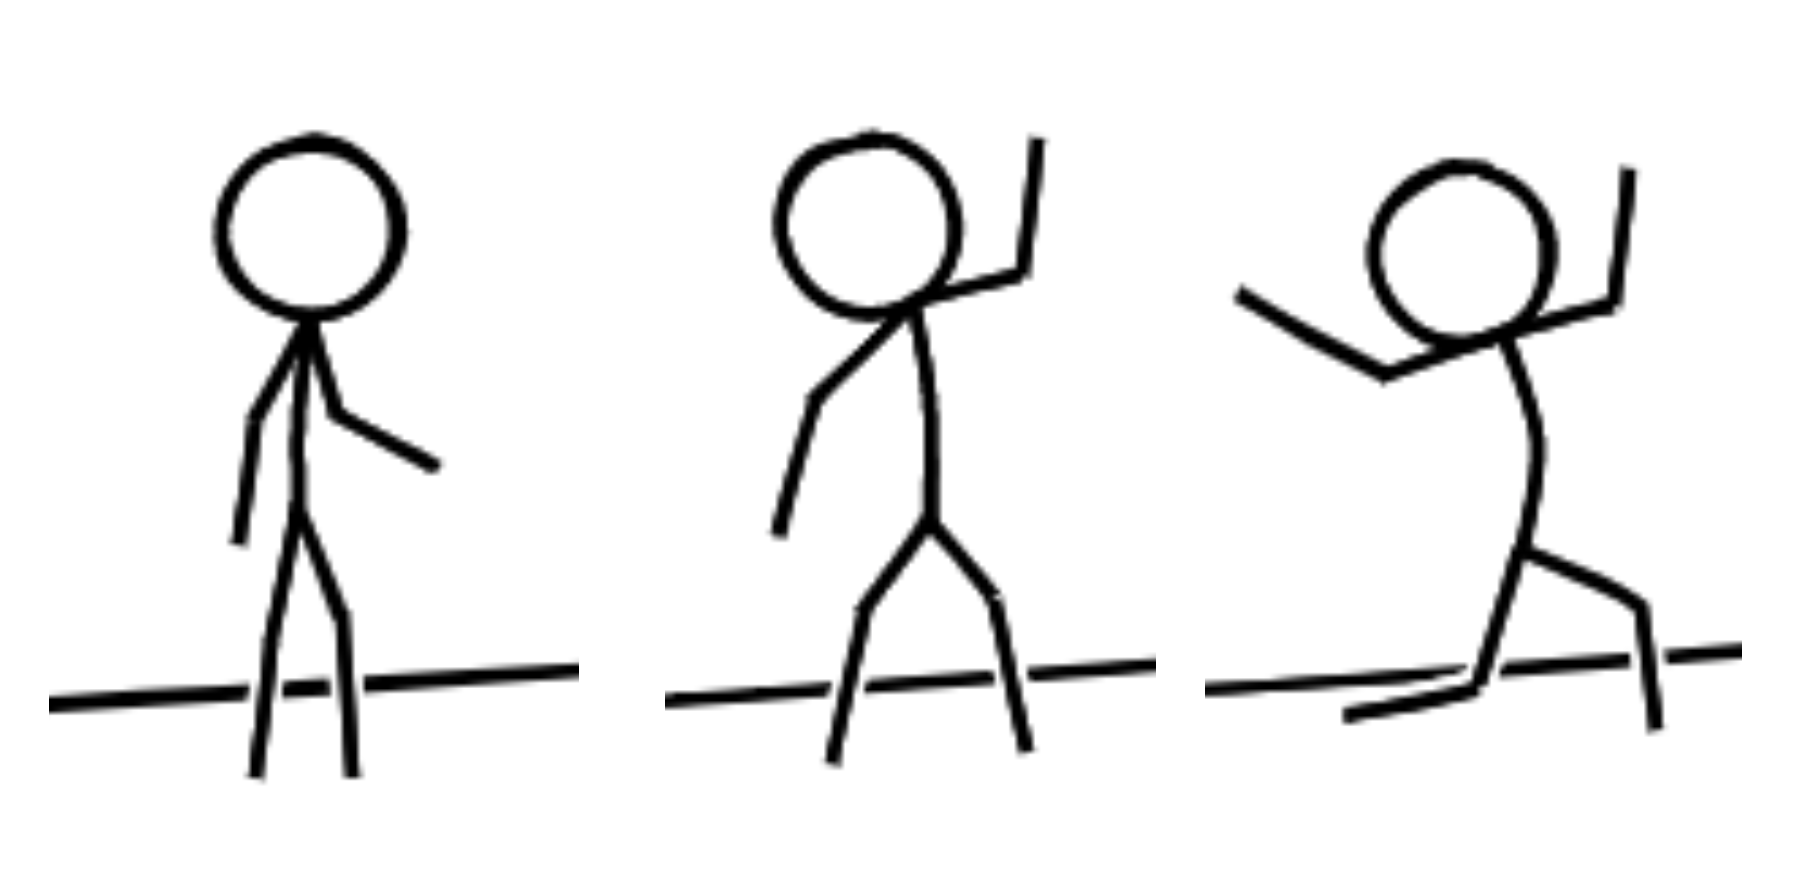
\includegraphics[width = 0.4\columnwidth]{figures/pos_figures}} &
        \subfloat[Gesture for negative framed messages ]{\label{figur:1b}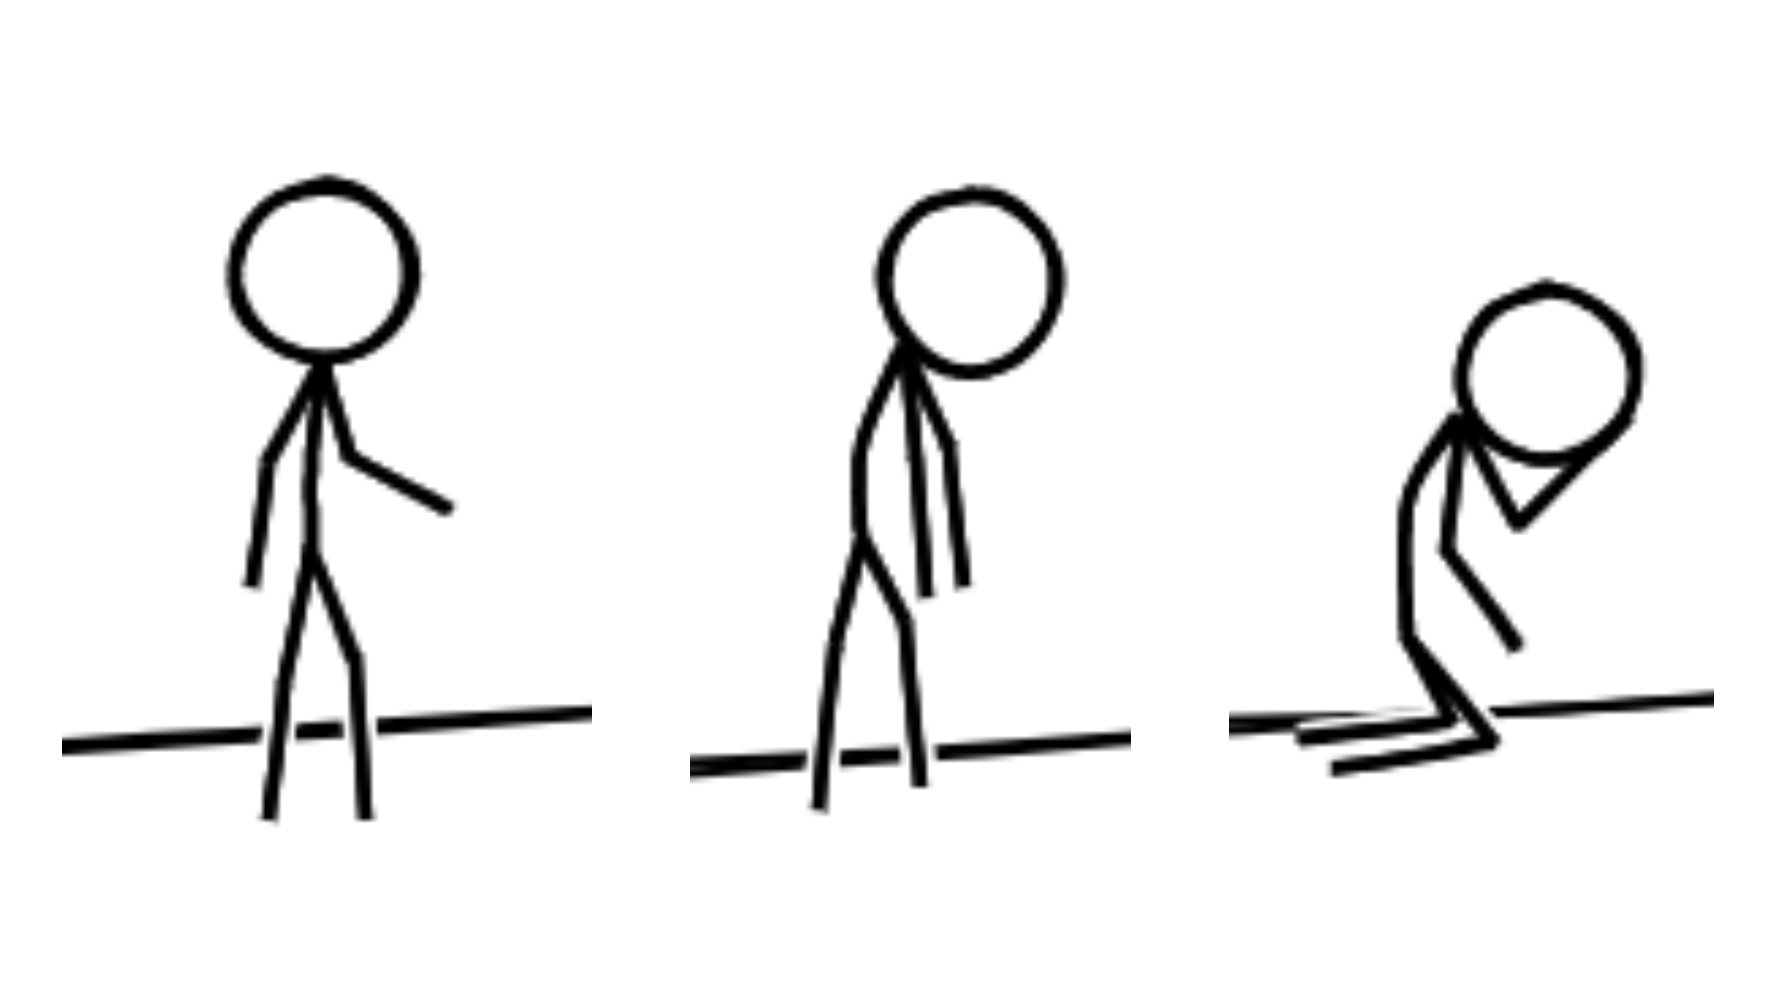
\includegraphics[width = 0.4 \columnwidth]{figures/neg_figures}}\\
    \end{tabular}
    \caption{Different character gestures to communicate various levels of emotional intensity. The left figure shows gestures from neutral to the happiest. The right figure shows gestures from neutral to the most frustrated. }
    \label{figur:figures}
\end{figure}

\subsection{Design Implications}
Our main design implications are two folded. First, when encouraging individuals to contribute to public goods, non-profit organizations and governmental agencies ought to consider to use abstract comic in their online messaging strategies to persuade. From our results, using abstract comics can, in particular, persuade people to act in public-goods dilemmas that require single-shot decisions (online charitable donations). Additionally, when constructing persuasive comics, it is worthwhile to consider to incorporate social norms. In the study, the purpose of the video is to inform participants about the context. Charities could use the comic after they've established context as discussed in~\Cref{sub:Experiments: Findings and Alternate Contexts}. 
% in the real world, the abstract comic message can be combined with campaign videos online to solicit donation.  Organizations can also consider to combine abstract comic messages with other introductory materials such as texts in an email or a physical mailer to persuade for contribution.

%; taking the flu shot
Second, our results also inform the development of a computational framework that can algorithmically synthesis textual persuasive messages into abstract comic form and uses data-driven methods to personalize the message to further increase messages' persuasive power. 
% With such a framework, agencies can create their abstract comic persuasive messages easily and incorporate them to alleviate real-world public goods dilemmas. 

\subsection{Limitations \& Future Work}
\begin{description}[leftmargin=\parindent,topsep=0pt,partopsep=3pt,parsep=0pt,itemsep=3pt, listparindent=\parindent]
\item[Distant and Non-exclusive Task:]  Although our study asked participants to make the decision with a real cost, the decision domain is limited to only one scenario, online charitable giving. In this task, the participant's reward is distant and non-exclusive (e.g., participant's donation decision won't bring any immediate reward and won't exclude the participant from the research outcome). Although both characteristics help us clearly test the persuasive benefits of abstract comics, they also limited our generalizability. We need future research to understand the pros and cons of using abstract comic messages in persuasive tasks with different reward characteristics. For example, for persuasive goals in the quantified-self movement~\cite{Epstein2014,Choe2014} such as exercise and dieting, the reward is distant (e.g., people's health won't be improved immediately after exercise) but exclusive (e.g., healthy life situation mainly benefit the individual him/herself). Moreover, our persuasion task is for an online charitable donation. Future work is needed to extend our result to offline charitable donation solicitation where persuasive text messages, such as mailers, also often used. 
\item[Study on Amazon Mechanical Turk:] We recruited our participants from Amazon Mechanical Turk, consistent with prior research \cite{lee2013does,saunders2016no,sussman2015framing,arechar2017turking,branas2018gender} that used Amazon Mechanical Turk subjects to study charitable donations. 


Although research shows that populations on Amazon Mechanical Turk are diverse and mirror the US population \cite{buhrmester2011amazon,behrend2011viability,berinsky2012evaluating}, there are concerns about Amazon Mechanical Turk's sample representativeness \cite{landers2015inconvenient,paolacci2010running}. One potential solution is to use panel population where the panel company claimed to offer a more diverse and representative sample.
However, this method also has concerns in that the researcher can not directly cross-validate the sample's representativeness we have to trust the company's assertion. Another solution is using stratified sampling, but it is challenging to classify every member of the population into a subgroup properly. 

Another limitation from use of Amazon Mechanical Turk subjects in our study is that prior research \cite{paolacci2010running,paolacci2014inside,kaufmann2011more} indicates that compared to other recruiting methods, study participants from Amazon Mechanical Turk are more sensitive to monetary rewards as monetary rewards are their prime motive for participation. 
% , compared to other recruiting methods, study participants from Amazon Mechanical Turk are more sensitive to monetary rewards. 
Since we ask our AMT study participants to donate from their own prospective rewards, we may see a lower average donation across all conditions, than for the population sample less sensitive to monetary rewards. An alternative sampling method we could consider in the future work is recruiting participants from our own social network. We conjecture that we may see higher average contributions in each of three conditions, since these participants may be less sensitive to monetary rewards than AMT participants. However, we need to carefully control for other potential confounding factors such as study participant's knowledge about our experiment goal. 
% What if we could recruit 
% such as the participant's own social network, we may expect a higher donation amount among all conditions. However, besides the potential sample representativeness problem (e.g. determining the size of participant's social network for the experiment), use of a social network introduces a confound: participants who are friends outside of the experiment may communicate outside of experimental communication channels.
% such sample may bring unexpected confounding factors such as their relationship with the researcher and knowledge about researcher's study topic. Additionally, \textcite{rzeszotarski2014estimating} showed that crowdsourcing may elicited higher quality results than friendsourcing on social networks

%  Prior research [51,50,32] indicates that compared to other recruiting methods, study participants from Amazon Mechanical Turk are more sensitive to monetary rewards as monetary rewards are their prime motive for participation. Since we ask AMT subjects to donate from their own prospective rewards, we may see a lower average donation across all conditions, than for the population sample less sensitive to monetary rewards.
  \item[Comic Message Construction:] In our study, we constructed the comic messages in the XKCD comic style. Although the XKCD style is easily recognizable, there are many different ways to create abstract comics.  Comic, as a creative art form, has rich semantics and vocabularies to communicate ideas \cite{scott1993understanding}. Out of necessity, we limited the complexity our comics strip (e.g., number of characters, gestures, and the number of panels). Future research is needed to explore and understand how other elements in the comic, for example, inter-character distance and character's gesture, affect the persuasiveness of the comic. Furthermore, while simplicity grants us the possibility to automate the generation process, future technology may allow us to generate more complicated persuasive abstract comics.
  
    \item[Other Experimental Contexts:] What are other contexts to which our study results may apply? Although our study examined charitable donation decisions, a single shot task with distant, non-exclusive rewards, certain health related tasks may be candidates to study next. Recent work by~\textcite{Bushar2017} on using SMS text messages to persuade pregnant mothers to take influenza vaccinations suggests that those who received the text messages were more likely to report taking a vaccination than those who did not receive a message. Further research is merited to determine if for this single-shot task, with exclusive, non-immediate reward, an abstract comic (e.g. embedded as a link in the SMS) succeeds in increasing vaccination rates for pregnant women over the plain text.
  
\end{description}

%need to update this part after the revision of RQ in the introduction
%Our experiment answers RQ-1 affirmatively in that comics are more persuasive than text, with a moderate effect of 0.33. Our answer to RQ-2 is that while the effect of no element is significant, shading and gesture show strong influence, but surprisingly inter-character distance is most effective when distance is large. For RQ-3, we show that negative messages are more influential than positive messages. We have developed a prototypical comic generator (answering RQ-4) that can be used in deploying comic messages.

%  \item[No interaction effects in the model]: Our model does not include any interaction effects. This is by design, since in the first study we have 54 experimental conditions making any analysis interaction effects difficult with our small observational study. The raw data suggest an interaction between shading and gesture, but given our limited dataset, there is little point in modeling this interaction. We plan to study interaction effects in future studies by limiting the number of main predictor conditions.
 %\item[Ecological Validity:] There is a legitimate question if our experiment on Amazon Mechanical Turk has ecological validity.  In real life, many factors affect a person's decision, such as where they are and who they are interacting with. Those factors may interact with the abstract comic's persuasiveness. However, these concerns are also present in other standard studies conducted in the more familiar lab experiments. We plan to conduct field studies in real-world contexts (e.g., shopping at a grocery store) to explore this issue.

% followed Our analysis shows that subjects prefer persuasive messages in comic form over plain text. We found in a persuasive comic, different character's gestures and background shading can influence subjects' perception of the persuasiveness whereas no strong effect was found in inter-character distance. This was consistent with previous research on visual stimulus in persuasion and the benefits of comics in communication.
%
% \subsection{Inter-Character Distance}
% \label{sub:Inter-Character Distance}
% There may be two explanations to the odd result that the farthest distance between the two characters was more influential.
% % However, previous studies on comics composition suggests the inter-character distance can affect reader's perceived relationship between characters and therefore influence their perception of the persuasive comics.
% First, it may be the case that the subjects did not project themselves onto the comic as one of the characters and did not recognize the distance between characters as reflecting closeness of the relationship. For example, a subject may read the comic from a third-person narrative. We looked into some feedbacks from in the pilot study. One participant ($p_1$) mentioned \textit{``I really like the comic I just saw and I feel bad that someone told me ...''} which suggests the subject does think that they are in the comic and having a conversation with someone else. Yet, we don't know if they perceive their relationship with the persuader based on the inter-character distance. A second explanation is that closer inter-character distance causes a cluttered visual composition and thus the subjects perceive these comics as less visually pleasing.

% \subsection{Comics with Color}
% \begin{figure}[t]
%  \centering
%  \begin{tabular}{ccc}
%   \subfloat[Colored Text]{\label{figur:3o}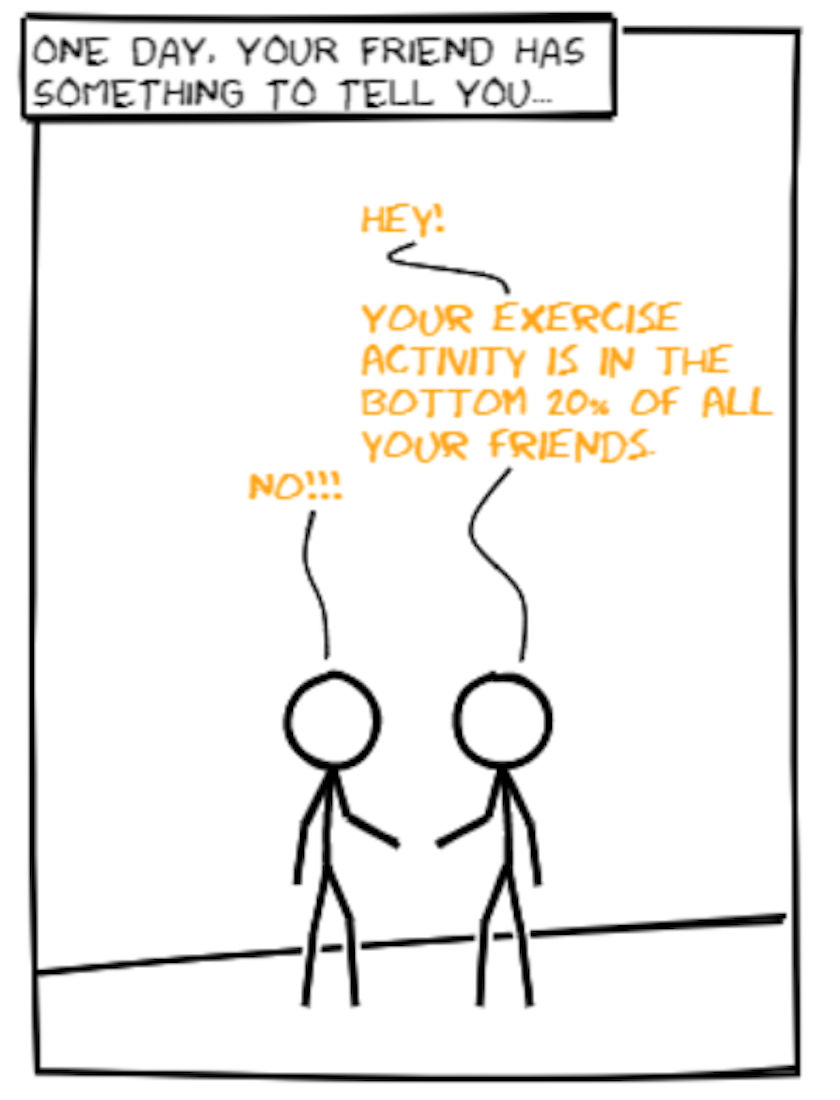
\includegraphics[width = 0.27\columnwidth]{figures/o1}} &
%   \subfloat[Colored Ground Line]{\label{figur:31}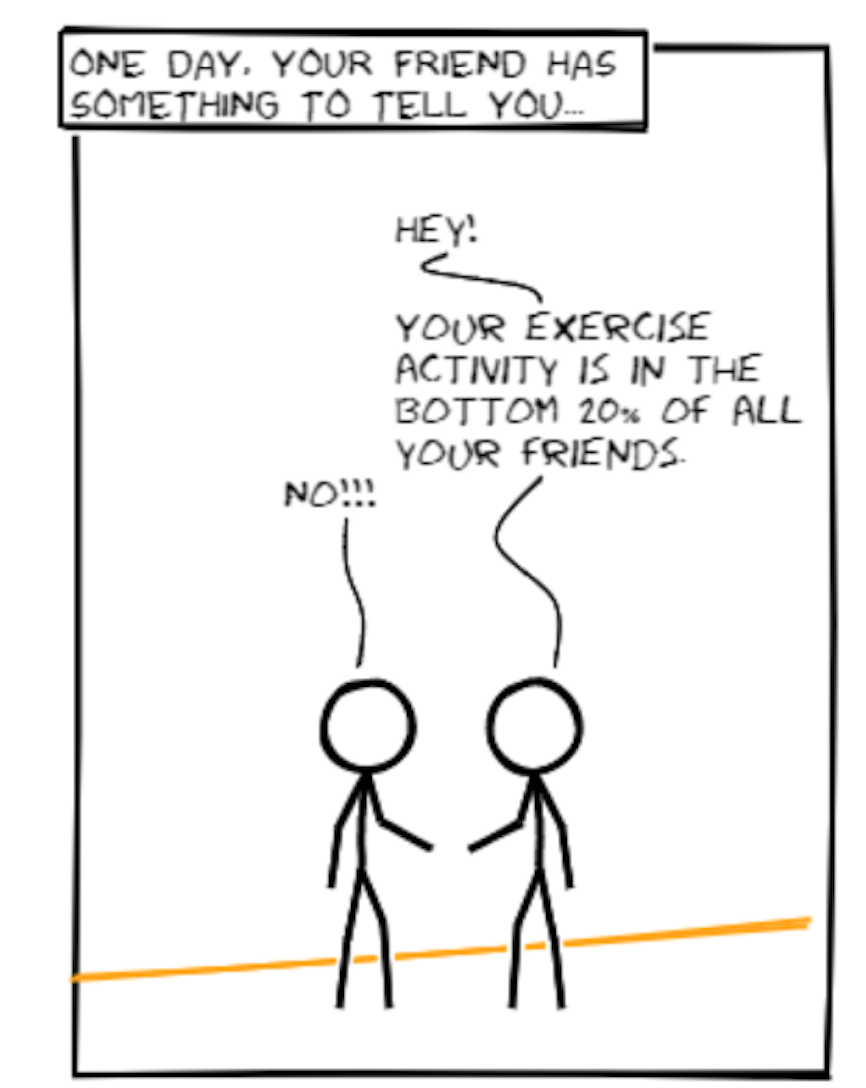
\includegraphics[width = 0.27 \columnwidth]{figures/o2}}      &
%   \subfloat[Colored Figure]{\label{figur:32}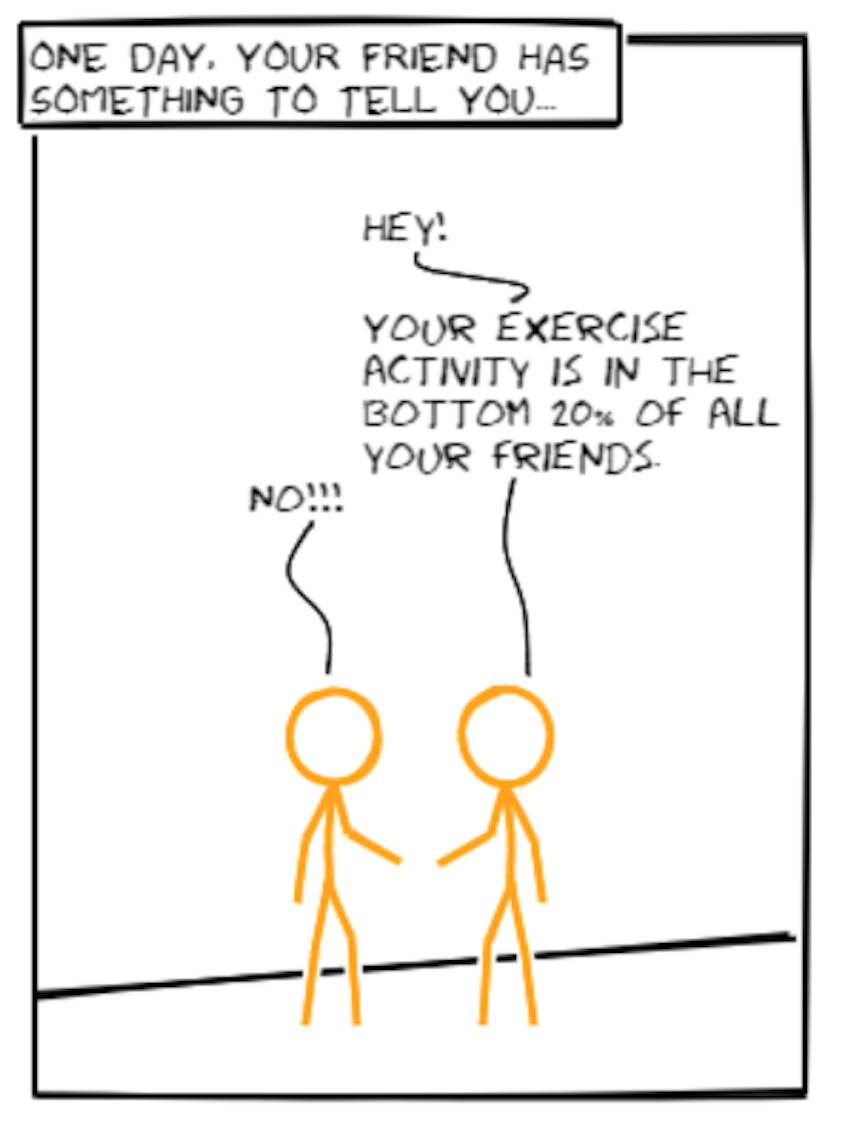
\includegraphics[width = 0.27 \columnwidth]{figures/o3}}\\
%  \end{tabular}
%  \caption{Colored different elements in a comic}
%  \label{figur:color}
% \end{figure}
%
% Our model suggests the background shading in a persuasive comic affects its persuasive power which makes us wonder the role of color as previous studies suggest the usage of color communicates the emotional intensity similar to the background shading. We ran a small scale study comparing the perceived persuasiveness between black-white comics in our study and their corresponding colored version,see figure~\ref{figur:color}. With 60 participants from the Mechanical Turk,  we found using an identical hierarchical Bayesian formulation that our subjects perceive colored version as more persuasive and there is potential interaction effect between negative-positive framing and different colors (see~\Cref{fig:color-experiment-effect}). We plan to run larger experiments that include color and study the interaction with framing and other elements.
%
% \begin{figure}
%  \subfloat[The mean effect and the effect size with color\label{subfig-1:color-mean-effect}]{%
%   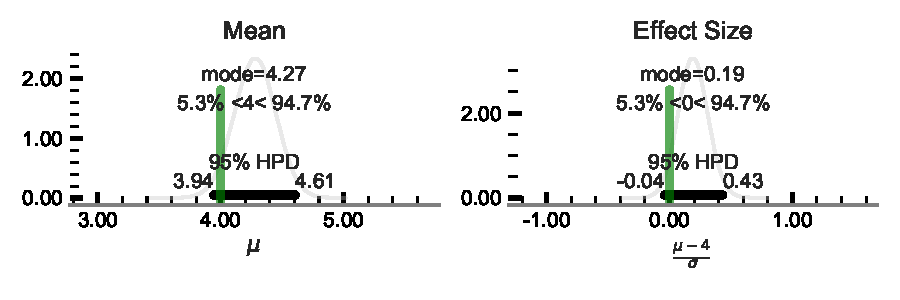
\includegraphics[width=0.6\textwidth]{./hari-code/factors_mean_effect_color-no-interaction.pdf}
%   } \hfill
%  \subfloat[Color contrast\label{subfig-2:color-contrast}]{%
%   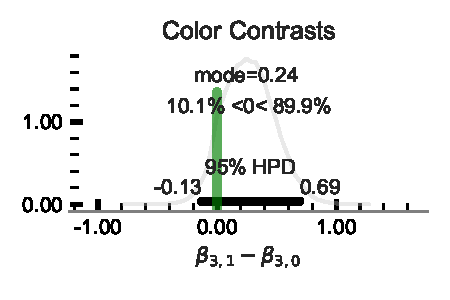
\includegraphics[width=0.33\textwidth]{./hari-code/factors_color_contrasts_color-no-interaction.pdf}
%  }
%  \caption{~\Cref{subfig-1:color-mean-effect} shows the High Posterior Density (HPD) intervals for the mean response $\mu$ and effect sizes $\sigma_y$ in the presence of color. HPD represent the region with 95\% of the density. Notice that the HPD interval for $\mu$ is $[3.94, 4.27]$ and includes a ROPE of $[4\pm 0.1]$ (the interval includes 4, the neutral response value). Thus while there no significant effect, we note that nearly 94\% of the HPD lies to the right of 0. The figure for effect size shows a small effect with mode $0.19$; since the HPD interval $[-0.04, 0.43]$ includes a ROPE of $[0\pm 0.1]$, there is no significant effect.~\Cref{subfig-2:color-contrast} shows the contrasts between the use of the two colors. The modal value is $0.24$, but since the HPD interval $[-0.13, 0.69]$ overlaps with 0, there is no appreciable effect (but notice that 89\% of the density lies in the region greater than 0.)}
%  \label{fig:color-experiment-effect}
% \end{figure}


%  Large scale field study is needed to demonstrate how the abstract comic can persuade in the real-life decision making and what will affect its persuasiveness.
 %Since we ask the subjects (who may lack interest in exercise) to evaluate persuasiveness when the topic is on exercise. Notice that our goal is not to persuade experimental subjects to exercise more, but to evaluate if the comic is a more persuasive form of communication of a statistical fact. We should expect---since we don't know if the subjects are interested in exercise---an increase in the variance in the estimates of the parameters (in particular,  $\sigma_y$). Despite this, the analysis shows a significant affirmative result for RQ-1.
%  \item[Appropriate gestures]: The authors determined gestures used by the characters in the experiment through trial and error. It may be useful to examine  theoretical frameworks from dance as well as theater art forms as well as examine work on design of sign languages.
% \end{description}
 % \item[Single Panel]: Our experiment limits our comics to a single panel which hinders one of the most fascinating aspect of comics---storytelling. Comparing to the comic strip, single panel comics find it harder to show the dynamic among characters.

%The main implication of our study lies in how to deliver persuasive messages. 

%Given the increasing popularity of wearable devices including smartwatches, one could consider presenting persuasive messages in the form of an abstract comic, where the three-panel comic is shown in sequence, perhaps even in animation. 

%Also, ~\textcite{scott1993understanding} identifies several fundamental components that influence reader reaction: character gestures, inter-character distance, and shading intensity. For example, the gesture of a character can help the reader to understand the interaction between characters and the emotion of the character. As a common technique, cartoonists often use the gesture to intensify the feeling that they want to communicate to the reader \cite{scott1993understanding}. Therefore, one of the future direction should be understanding how the different comic components moderate comic persuasiveness. If different comic elements car persuades differently, taking advantage of data-driven methods, the abstract-comic can better persuade. To maximize the persuasive power, future research on computational persuasion should leverage the receiver's personal model to construct the persuasive abstract comics with elements best fit to the persuadee.
